\documentclass{article}
\usepackage[utf8]{inputenc}
\usepackage{graphicx}

\setlength{\parindent}{0pt}
\usepackage[letterpaper, margin=1.0in]{geometry}

\title{MATH 115: Applications of Optimization Problems}
\author{Sam Boardman}
\date{March 20, 2024}

\begin{document}

\maketitle

\section{Introduction}

The purpose of this document is to offer students more interesting and varied optimization problems than otherwise possible in a calculus course by introducing domain knowledge from several disciplines that often find use for mathematics. The problems may be attempted in any order based on the reader's own interests. Problems marked by (\textasteriskcentered{}) are more challenging (or more abstract) than optimization questions likely to appear on an exam for MATH 115. 

\newpage

\section{Statistics}

\begin{enumerate}

    \item One goal of \textit{descriptive statistics} is summarizing a dataset (which, for us, is a list of numbers) by a single number that best describes it. One way to do this is by defining some notion of distance to the dataset, then taking the number that minimizes this distance.

    \begin{enumerate}
    
        \item Let $a$, $b$, and $c$ be real numbers and consider the function $f(x) = (a-x)^2 + (b-x)^2 + (c-x)^2$, the sum of squared distances from each of the above numbers to $x$. Show that the global minimum of $f$ occurs at $x = \frac{a+b+c}{3}$, the mean of $a$, $b$, and $c$.

        \vfill 

        \item Using the sum rule and your answer to (a), explain why for any real numbers $a_1,a_2,\dots,a_n$, the function $f(x) = (a_1-x)^2 + (a_2-x)^2 + \cdots + (a_n-x)^2$ attains its global minimum at $x = \frac{a_1 + a_2 + \cdots + a_n}{n}$, the mean of $a_1,a_2,\dots,a_n$. 

        \vfill

        \item Let $a$, $b$, and $c$ be real numbers such that $a \leq b \leq c$ and consider the function $g(x) = |a-x| + |b-x| + |c-x|$, the sum of distances from each of the above numbers to $x$. Show that the global minimum of $g$ occurs at $x = b$, the median of $a$, $b$, and $c$. 

        \vfill 

        \item (\textasteriskcentered{}) Extending the reasoning from (c), show that for any real numbers $a_1,\dots,a_n$ such that $a_1 \leq a_2 \leq \cdots \leq a_n$, the function $g(x) = |a_1-x| + |a_2-x| + \cdots + |a_n-x|$ attains its global minimum at $x = a_{(n+1)/2}$ if $n$ is odd and every number in the interval $[a_{n/2},a_{n/2+1}]$ if $n$ is even (such a number is called \textit{a} median of $a_1,a_2,\dots,a_n$).

        \vfill 

        \item (\textasteriskcentered{}) Using the second derivative of the above functions (or terms thereof) and the results of (b) and (d), explain why the mean is considered more sensitive to outliers in a dataset than the median.  

        \vfill

    \end{enumerate}

    \newpage

    \item In \textit{inferential statistics}, the focus is instead on using a sample of data to draw conclusions about an underlying distribution. If a coin that lands heads with probability $p$ is tossed 20 times independently, then the probability it lands heads 16 times is $4845p^{16}(1-p)^4$. What value of $p$, where $0 \leq p \leq 1$, results in the largest probability of the coin landing heads 16 times as above? (We can use this value to estimate $p$; this is called \textit{maximum likelihood estimation}.) 

    \vfill 

\end{enumerate}

\section{Machine Learning}

\begin{enumerate} 
    \addtocounter{enumi}{2}

    \item A popular paradigm for machine learning is \textit{supervised learning}, where we are given a list of points in the plane, $(x_1,y_1),\dots,(x_n,y_n)$, and the goal is to learn how to predict the $y$-values of new points when we are just given their $x$-values. For instance, each point $(x,y)$ may correspond to a song a user has listened to on Spotify, where $x$ is a proprietary score representing how transformative the bridge is, and $y$ is a score representing how much the user likes the song (based on searches, replays, etc.). Now the app's recommendation system needs to give the user songs they haven't heard before, and a simplified approach to doing so is using the songs' bridges to predict how much they'll like certain songs, then recommend the ones that get the highest scores. \\

    One way to predict $y$-values from $x$-values is \textit{least-squares linear regression}: model $y$ as a linear function of $x$, i.e. $\hat{y}(x) = mx+b$, where $m$ and $b$ are chosen to minimize the sum of squared distances $L$ between the actual $y$-values and those predicted by a linear function based on the $x$-values: $L = (y_1-\hat{y}(x_1))^2 + (y_2-\hat{y}(x_2))^2 + \cdots + (y_n-\hat{y}(x_n))^2$.    

    \begin{enumerate}
        \item (\textasteriskcentered{}) Let $m$ be a constant. In terms of $m$, what value of $b$ minimizes the number $L$ as defined above? \\
        \textit{Hint:} Draw some points in the plane along with a line that lies above some of the points and below others. How does shifting the line vertically affect $L$? See if you can apply one of the results from problem 1 instead of taking another derivative. 

        \vfill

        \item (\textasteriskcentered{}) Using your answer to (a), find the value of $m$ and $b$ that minimize the number $L$ as defined above.

        \vfill
    \end{enumerate}

    \newpage

    \item (\textasteriskcentered{}) Problem 3 concerned one major part of supervised learning tasks: optimization. It turns out, however, that if we consider too many ways to model $y$ as a function of $x$, then we can almost always find a function that passes through all of the points $(x_1,y_1),\dots,(x_n,y_n)$. This is called overfitting, and often results in a model that does a poor job of predicting the $y$-values of previously unseen $x$-values. Thus, another critical part of supervised learning is generalization: ensuring that with high probability, a model that has low error in estimating $y_1,\dots,y_n$ will also have low error in estimating new $y$-values, which is done by restricting the expressive power of the set of functions $H$ we optimize over, denoted by $R(H)$. \\

    For a given supervised learning problem, it is known that for any constant $\lambda > 0$, $R(H) \leq \frac{1}{\lambda}g(H) + \frac{\lambda}{2n}$, where $g$ is a positive function. Show that $R(H) \leq \sqrt{\frac{2g(H)}{n}}$. 

    \vfill
    
\end{enumerate}

\section{Economics}

\begin{enumerate}
    \addtocounter{enumi}{4}
    
    \item A fancy restaurant, {\sc Eats4U}, holds a wine tasting event. If $p$ is the price of admission in dollars, then previous experience suggests that the demand can be modeled as $d(p) = 1000p^{-1/3}e^{-.01p}$, meaning that a total of $d(p)$ (21+) people will pay for admission if there is room for them at the restaurant. Suppose that the restaurant has room for 250 people in total. 

    \begin{enumerate}
        \item (\textasteriskcentered{}) Suppose that under a previous price $p_0$, $d(p_0) > 250$. Using continuity of $d$, explain why the restaurant can increase the price while still admitting 250 people for the event.

        \vfill

        \item What price of admission maximizes the amount of money collected from customers (i.e. revenue) for the event?

        \vfill
    \end{enumerate}

    \newpage

    \item Braess's paradox is the counterintuitive observation that adding roads or lanes to a driving infrastructure can increase the travel time of all drivers if they act in their own self-interest. Consider the networks of roads shown in Figure \ref{braesss_paradox}. In this problem, we evaluate the performance of each network in taking people from $s$ to $t$. More formally, if $x$ is the fraction (e.g. $.4 = 40\%$) of people that use a given road on their route, then the travel time for that road is given by the function $c(x)$ written above that edge. The average travel time is the sum of the travel time for each road times the fraction of people that use that road on their route.

    \begin{figure}[h]
        \centering
        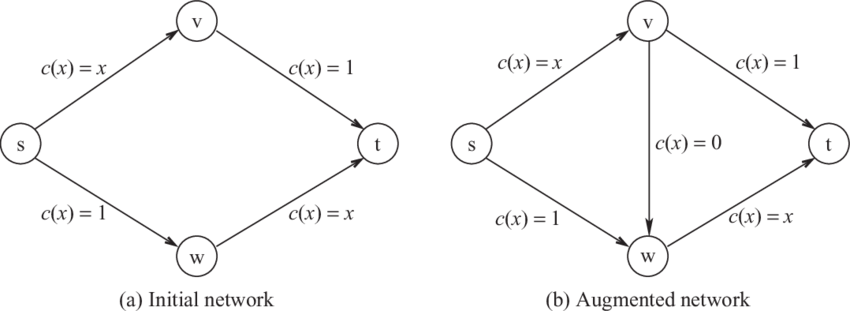
\includegraphics[scale=.95]{braesss_paradox.png}
        \caption{Two networks of roads, where $s$, $t$, $v$, and $w$ are junctions and the four or five line segments connecting them are roads. In Network (a), the only routes from $s$ to $t$ are $s \to v \to t$ and $s \to w \to t$. In Network (b), an ultrafast shortcut is added between $v$ and $w$ that always has a travel time of 0, creating an additional route from $s$ to $t$ of $s \to v \to w \to t$.}
        \label{braesss_paradox}
    \end{figure}

    \begin{enumerate}
        \item The socially optimal average travel time is the minimum possible average travel time. Find the socially optimal average travel time in Network (b) by using the fact that achieving it does not require using the shortcut from $v$ to $w$.

        \vfill

        \item A \textit{Nash equilibrium} in the context of this problem is an assignment of drivers to routes from $s$ to $t$ in the network so that no (fraction of) drivers would attain a lower travel time by switching to another route. It can be shown that any Nash equilibrium in Network (a) has 50\% of drivers on the upper route and 50\% of drivers on the lower route. In Network (b), where the shortcut is added, the Nash equilibrium has 100\% of drivers cutting across this shortcut, which actually increases the travel time for everyone! \\

        In Network (b), compute the ratio of average travel time in the Nash equilibrium to the socially optimal average travel time. (This is called the \textit{price of anarchy}; people designing networks are interested in this being as close to 1 as possible, meaning that selfish behavior does not degrade system performance that much.) How does this compare to Network (a)? 

        \vfill
    \end{enumerate}

    
\end{enumerate}

\newpage

\section{Physics}

\begin{enumerate}
    \addtocounter{enumi}{6}

    \item Inspired by his father's early career, Sam moves to Australia and becomes a full-time lifeguard, feeling wistful for his past life as a mathematician whenever the sinusoidal oscillation of the water level erodes a child's sandcastle. Suppose that at a particular moment, the water is 5 meters east of the lifeguard stand and runs north-to-south.  

    \begin{enumerate}
        \item Using a buoy as a point of reference, Sam notices a swimmer in distress 30 meters east and 6 meters north of the lifeguard stand. Suppose Sam can move at a speed of 7 meters/second on the sand and 1.5 meters/second in the water. At what point should Sam enter the water to minimize the amount of time it takes to reach the swimmer? \\
       \textit{Hint:} For any line segment that lies entirely in the sand or in the water, one can compute the amount of time it takes to travel across it by dividing its length by the velocity in that region.  

        \vfill 

        \item (\textasteriskcentered{}) Reasoning more abstractly and using that light takes the fastest path when traveling between two points, prove Snell's law: if light (Sam) travels at a velocity of $v_1$ in one medium (sand) and $v_2$ in the second (water), and $\theta_1$ and $\theta_2$ are the corresponding angles the ray of light (Sam's path) in that medium forms with a line perpendicular to the interface of the media (the waterline), then $v_1\sin\theta_2 = v_2\sin\theta_1$.    

        \vfill 
    \end{enumerate}
    
\end{enumerate}

    
\end{document}
